%\appendix{Представление графического материала}

Графический материал, выполненный на отдельных листах,
изображен на рисунках А.1--А.\arabic{числоПлакатов}.
\setcounter{числоПлакатов}{0}

\renewcommand{\thefigure}{А.\arabic{figure}} % шаблон номера для плакатов

\begin{landscape}
\begin{плакат}
	\centering
    \includegraphics[width=0.8\linewidth]{вкрб}
    \заголовок{Сведения о ВКРБ}
    \label{pl1:image}      
\end{плакат}

\begin{плакат}
	\centering
    \includegraphics[width=0.8\linewidth]{цели}
    \заголовок{Цель и задачи разработки}
    \label{pl2:image}      
\end{плакат}

\begin{плакат}
	\centering
    \includegraphics[width=0.8\linewidth]{концепт}
    \заголовок{Концептуальная модель сайта}
    \label{pl3:image}      
\end{плакат}

\begin{плакат}
	\centering
    \includegraphics[width=0.8\linewidth]{umlshema}
    \заголовок{Диаграмма прецедентов}
    \label{pl4:image}      
\end{плакат}

\begin{плакат}
	\centering
	\includegraphics[width=0.8\linewidth]{компонент}
	\заголовок{Диаграмма компонентов}
	\label{pl5:image}      
\end{плакат}

\begin{плакат}
	\centering
	\includegraphics[width=0.8\linewidth]{регистрация}
	\заголовок{Страница регистрации и авторизации}
	\label{pl6:image}      
\end{плакат}

\begin{плакат}
	\centering
	\includegraphics[width=0.8\linewidth]{главная_1}
	\заголовок{Главная страница}
	\label{pl7:image}      
\end{плакат}

\begin{плакат}
	\centering
	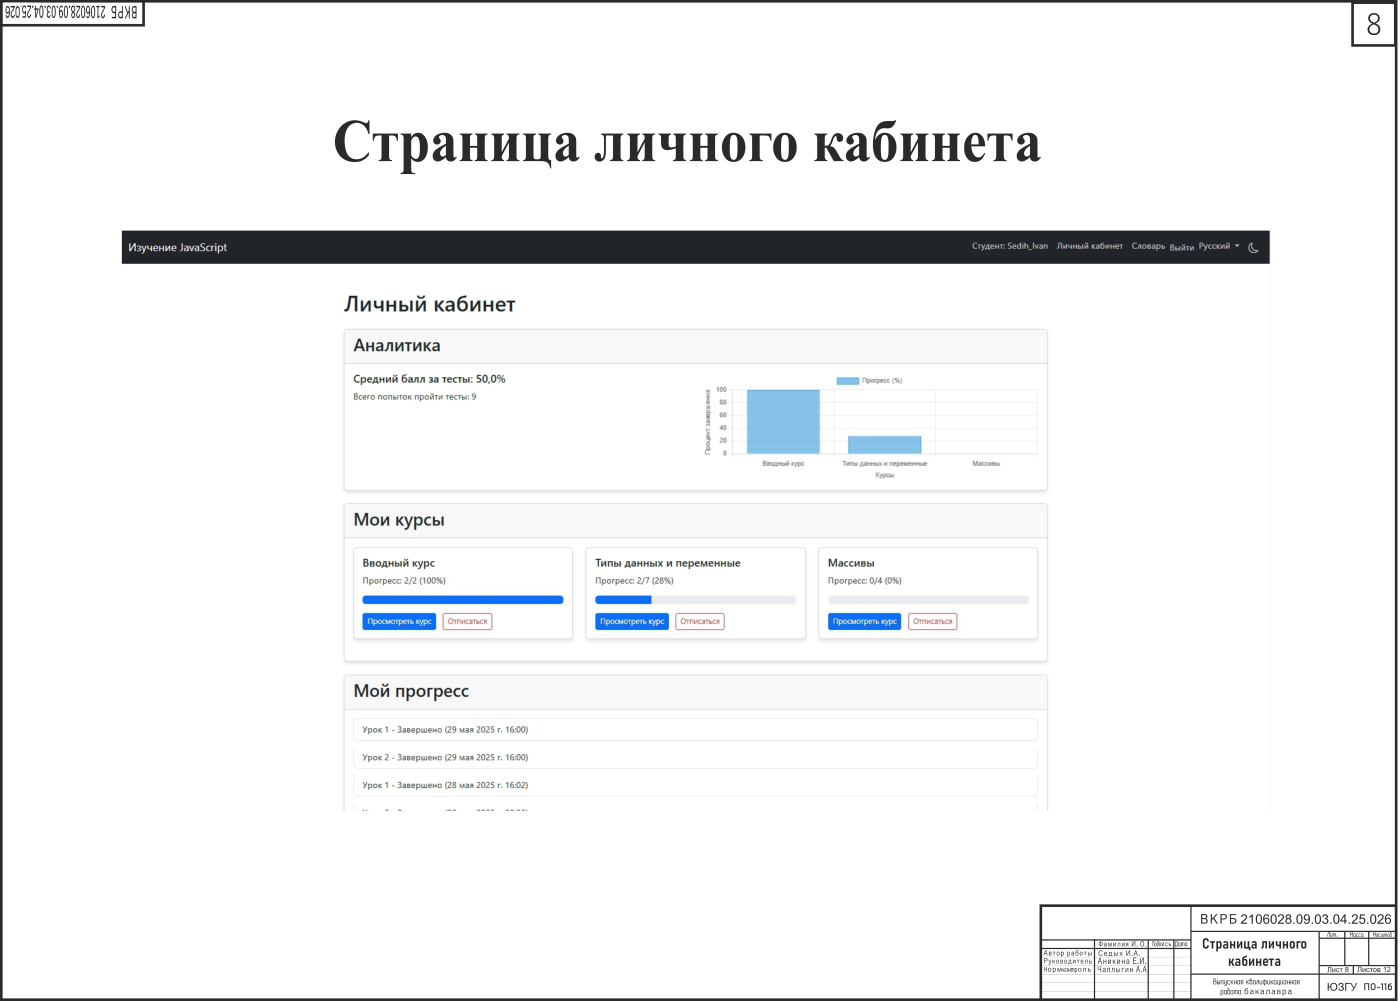
\includegraphics[width=0.8\linewidth]{кабинет}
	\заголовок{Личный кабинет}
	\label{pl8:image}      
\end{плакат}

\begin{плакат}
	\centering
	\includegraphics[width=0.8\linewidth]{добавитьурок}
	\заголовок{Страница добавления урока}
	\label{pl9:image}      
\end{плакат}

\begin{плакат}
	\centering
	\includegraphics[width=0.8\linewidth]{словарь1}
	\заголовок{Страница словаря}
	\label{pl10:image}
\end{плакат}

\begin{плакат}
	\centering
	\includegraphics[width=0.8\linewidth]{резытеста}
	\заголовок{Страница результатов тестов}
	\label{pl11:image}      
\end{плакат}

\begin{плакат}
	\centering
	\includegraphics[width=0.8\linewidth]{заключение}
	\заголовок{Заключение}
	\label{pl12:image}      
\end{плакат}
\end{landscape}
